Ray tracing is a technique for generating 3D computer graphics that attempts to simulate the behavior of light in real life. Due to its ability to accurately model light transport, ray tracing is widely used in animated movies and VFX to generate photorealistic images. Recent advances in hardware acceleration have made ray tracing a viable alternative to rasterized rendering for games and other performance sensitive tasks. Since its inception in 1971, it remains one of the simplest and most intuitive ways to generate 3D images and serves as a classic introduction to the mathematical foundations of computer graphics.
\begin{figure}[h]
    \centering
    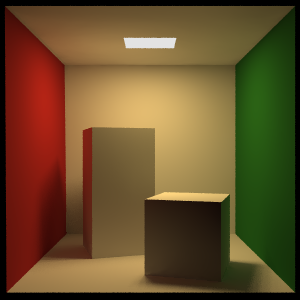
\includegraphics[scale=0.7]{figures/Cornell_box.png}
    \caption{The Cornell Box, a commonly used test scene for ray tracers showcasing indirect lighting capabilities (Wikimedia Commons)}
    \label{fig:cornell_box}
\end{figure}
\\
\noindent
This article will be fairly light on implementation details, focusing more on the theory of ray tracing. Nonetheless, the information should be sufficient to implement your own basic ray tracer in a language of your choice with simple shading, shadows, and reflections.